\section{Ejercicio 1}

En este ejercicio nos dan la triangulación de un polígono y a partir de la misma recuperar el polígono original. En la entrada se nos da los extremos de cada uno de esos triángulos pero uno a partir de ello podría dibujar todos los triángulos y formar la figura original. La cantidad de lados del polígono es n, con lo cual la cantidad de triángulos en la entrada es n-2.\newline

Un ejemplo podría ser el siguiente:\newline

\begin{figure}[h!]
	\centering
	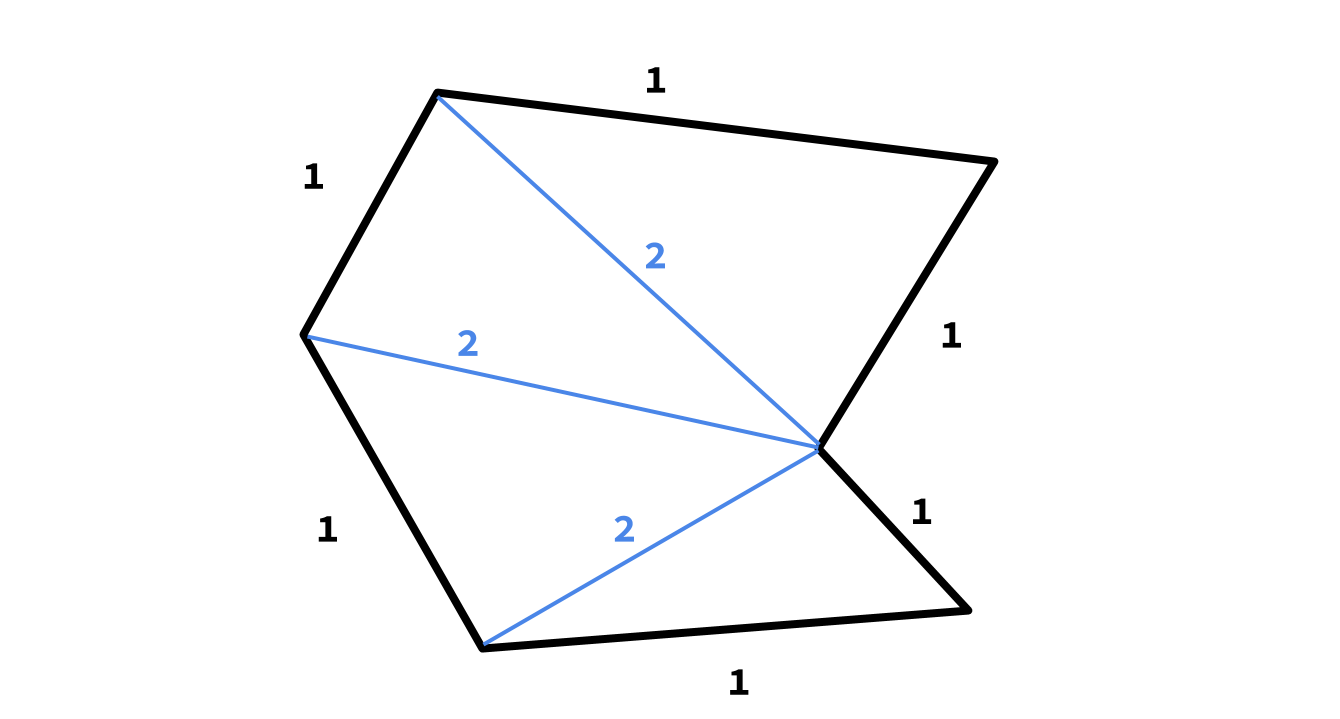
\includegraphics[scale = 0.25]{img/poligono-triangulado.png}
\end{figure}

Los números que hay sobre cada uno de los lados son la cantidad de veces que uno tuvo que dibujar dicho segmento para cada triángulo de la entrada.\newline

No es casualidad que los lados del polígono hubo que dibujarlas una única vez y los lados de los triángulos que son internos en el polígono dos veces.\newline

\textbf{AGREGAR JUSTIFICACION FORMAL; NO SE ME OCURRE UNA.}\newline

Esta observación nos da un algoritmo para poder generar el polígono original.\newline

\begin{algorithmic}

\Function{diferenciar_lados}{lista [triángulo] triángulos}{lista[lado]}
	\State mapa \{lado, veces\} veces_usado $\gets$ \{\}
	\For {triángulo t : triángulos}
		\For{lado l : lados[t]}
			\State veces_usados[l] $\gets$ veces_usados[l] + 1
		\EndFor
	\EndFor 
	\State lado lados_polígono [] $\gets$ []
	\For {(lado,veces) tupla: veces_usado}
		\If tupla.veces $=$ 1
			\State Agregar(tupla.lado, lados_poligono)
		\EndIf
	\EndFor
	\State \Return lados_polígono
\EndFunction

\end{algorithmic}

Solamente nos falta devolver dichos lados en sentido horario.\newline

Para eso podemos podemos pensar de la siguiente manera: como tenemos un polígono, para cada uno de los vértices vamos a tener dos vértices incidentes, con lo cual tenemos dos vértices vecinos.\newline

Luego, podemos tomar un punto arbitrario de los que tenemos y hacemos el producto cruz entre los vectores que nos definen los segmentos que se generan con los dos vecinos al punto. Como bien vimos en clase, el signo del producto cruz entre dos vectores nos determina si el segundo vector está a la izquierda o bien a la derecha del primero (en nuestro caso no puede dar cero al no haber puntos colineales).Si dicho punto arbitrario es el que está más abajo a la izquierda de todos los del polígono, tomar el segmento que se define con los vecinos que está a la izquierda del otro podemos asegurar que al moverse a partir de ahí en adelante el sentido que tomaremos será horario. En la siguiente figura se refleja lo planteado anteriormente.

\begin{figure}[h!]
	\centering
	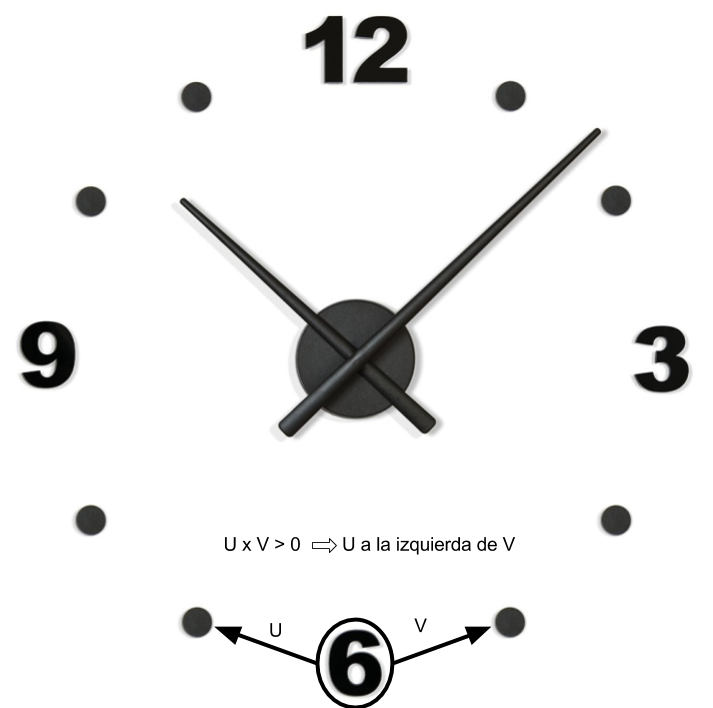
\includegraphics[scale = 0.25]{img/sentido-horario.png}
\end{figure}

Con lo cual empezamos a recorrer el polígono a partir de este segmento que tomamos y a través de los lados del polígono nos movemos hasta llegar nuevamente hasta el origen y así tenemos nuestro polígono recorrido en sentido horario.\newline    

Esto lo logramos a partir de un recorrido de dfs en el grafo inducido que nos da el polígono.\newline

\begin{algorithmic}

\Function{lados_sobre_vertices}{lista [lado] lados}{mapa\{punto, lista[punto]\}}
	\State mapa \{punto, lista[lado]\} segmentos_incidentes $\gets$ \{\}
	\For {lado lado : lados}
		\State segmentos_incidentes[lado.extremo1].agregar(lado.extremo2)
		\State segmentos_incidentes[lado.extremo2].agregar(lado.extremo1)
	\EndFor 
\EndFunction
\end{algorithmic}


\begin{algorithmic}
\State solución $\gets$ []

\Function{recorrer_y_agregar}{vértice_actual, vertice_anterior, mapa\{punto, lista[punto]\}segmentos_incidentes, inicial}{}
	\State Agregar(vertice_actual, solución)
	\If{segmentos_incidentes[vértice_actual][0] $=$ vertice_anterior}
		\If{segmentos_incidentes[vértice_actual][1] $\neq$ inicial}
			\State recorrer_y_mostrar(segmentos_incidentes[vértice_actual][1], actual, segmentos_incidentes, inicial)
		\EndIf
	\Else
		\If{segmentos_incidentes[vértice_actual][0] $\neq$ inicial}
			\State recorrer_y_mostrar(segmentos_incidentes[actual][0], actual, segmentos_incidentes, inicial)
		\EndIf
	\EndIf
\EndFunction

\end{algorithmic}

\subsection{Cumpliendo la complejidad pedida}
Para poder cumplir con la complejidad pedida utilizamos el map de la stl que tarda tiempo logarítmico al insertar o consultar un elemento tanto para los lados de los triángulos como para los lados incidentes a los vértices del polígono.\newline

La cantidad de lados que insertamos y luego le consultamos la cantidad de usos son en total 3 * (n-2) con lo cual tenemos \bigo(n) lados. Si por cada uno aplicamos operaciones de tiempo logarítmico, encontrar cuales lados pertenecen al polígono nos cuesta \bigo(n $\times$ log n).\newline

Luego por cada uno de los lados, marcamos en el mapa de puntos a qué dos puntos es incidente tardando nuevamente \bigo(n $\times$ log n) al ser n + 1 la cantidad de vértices de nuestro polígono.\newline

Finalmente hacer el producto cruz entre dos segmentos nos cuesta \bigo(1) pero recorrer los n lados del polígono nos cuesta en total \bigo(n $\times$ log n) al ser estos n+1 elementos y consultar cuáles son los dos vecinos a éste nos cuesta tiempo logarítmico al estar insertados en un mapa.\newline

La complejidad total de nuestro algoritmo nos queda entonces \bigo(n $\times$ log n).\newline